\section{Additional Experiment Results}
\label{appendix:addition_experiments_results}

\begin{figure}[ht]
    \centering
    \begin{subfigure}[t]{0.33\textwidth}
        \centering
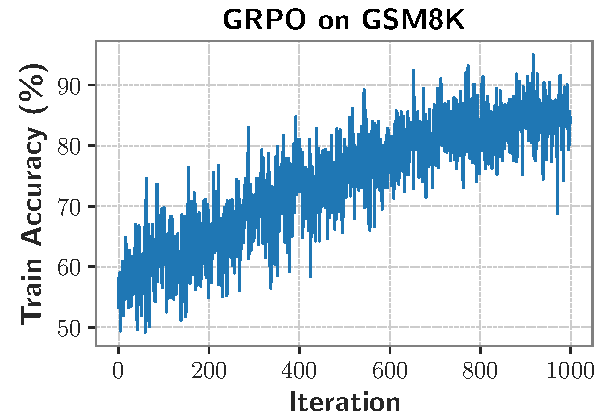
\includegraphics[width=\textwidth]{eval-figures/GRPO-overfit-train-acc.pdf}
        \caption{Train Accuracy.}
        \label{fig:grpo-train-accuracy}
    \end{subfigure}% 
    \hfill 
    \begin{subfigure}[t]{0.33\textwidth}
        \centering
        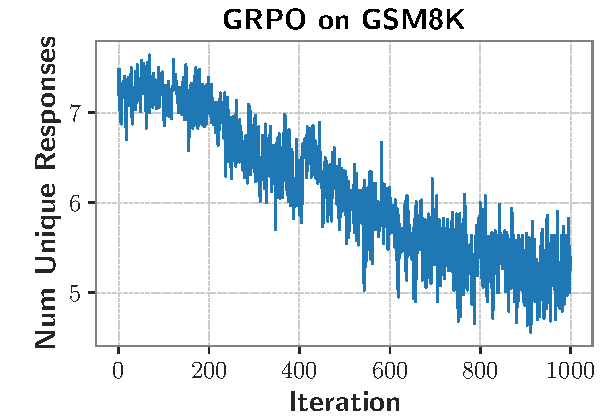
\includegraphics[width=\textwidth]{eval-figures/GRPO-overfit-train-num-response.pdf}
        \caption{Train Num Unique Responses.}
        \label{fig:grpo-train-num-unique-responses}
    \end{subfigure}
    \hfill
    \begin{subfigure}[t]{0.33\textwidth}
        \centering
        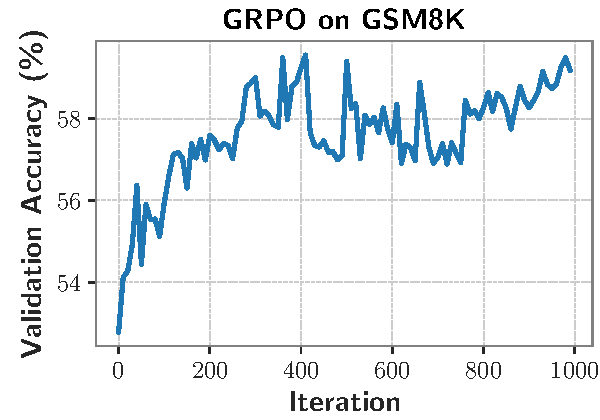
\includegraphics[width=\textwidth]{eval-figures/GRPO-overfit-val-acc.pdf}
        \caption{Validation Accuracy.}
        \label{fig:grpo-val-accuracy}
    \end{subfigure}%
    \caption{GRPO on GSM8K exhibits rapid overfitting: while training accuracy improves steadily (Fig. \ref{fig:grpo-train-accuracy}), but the unique response number constantly drops (Fig. \ref{fig:grpo-train-num-unique-responses}), and validation accuracy saturates early (Fig. \ref{fig:grpo-val-accuracy}).}
    \label{fig:grpo_overfit}
\end{figure}

We also evaluate our SPO-chain method using DeepSeekMath 7B on the MATH dataset, as shown in Figure~\ref{fig:deepseek_math_7b}. Our approach achieves performance comparable to VinePPO and surpasses all other baselines. Due to computational constraints, we initially train with an interval of 10 and later switch to 5. After switching from the interval of 10 to 5, the model performance continues to improve, suggesting that using a finer-grained advantage is beneficial for model training. Notably, as shown in Figure \ref{fig:deepseek_math_7b_num_sampling_points}, our method uses significantly fewer segments than VinePPO while attaining similar performance.

\begin{figure}[ht]
\centering
\begin{minipage}{0.48\textwidth}
  \centering
  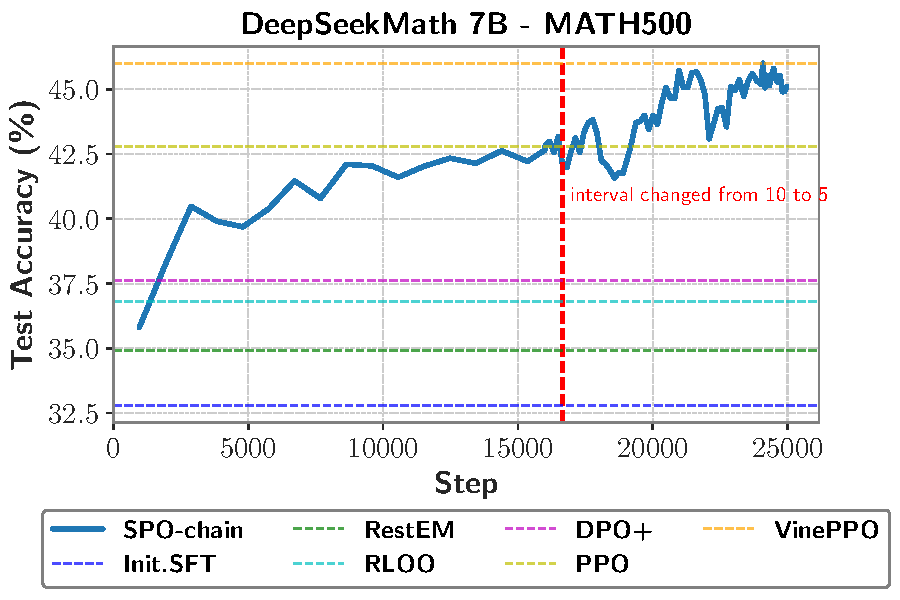
\includegraphics[width=\linewidth]{eval-figures/deepseek-math-7b.pdf}
  \caption{Performance of SPO-chain on DeepSeekMath 7B evaluated on the MATH500. Baseline results are from \cite{kazemnejad2024vineppounlockingrlpotential}.}
  \label{fig:deepseek_math_7b}
\end{minipage}
\hfill
\begin{minipage}{0.48\textwidth}
  \centering
  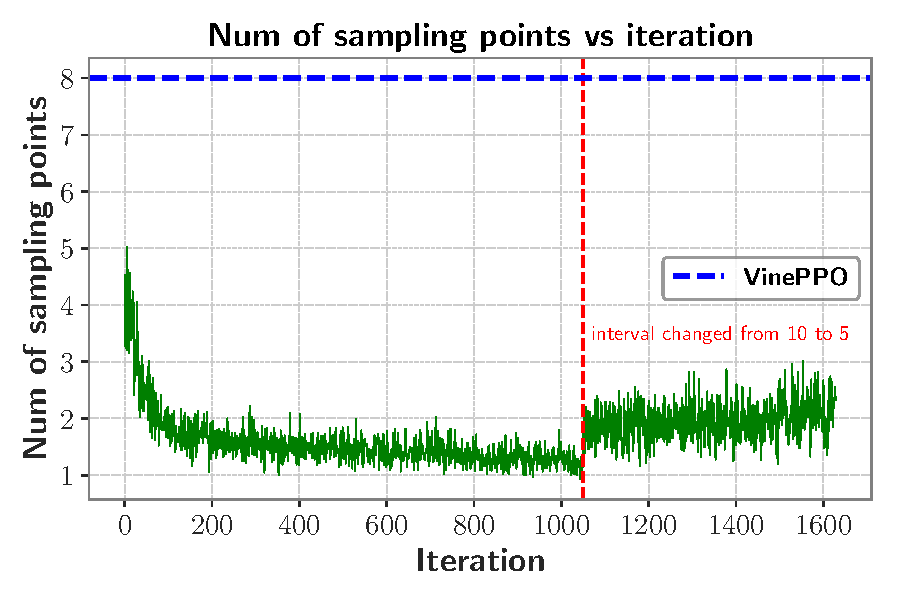
\includegraphics[width=\linewidth]{eval-figures/deepseek-math-7b-num-sampling-points.pdf}
  \caption{Comparison of the number sampling points between our method and VinePPO. According to \cite{foster2025learningreasonfrontierlearnability}, there are approximately 8 reasoning steps on average for MATH.}
  \label{fig:deepseek_math_7b_num_sampling_points}
\end{minipage}
\end{figure}

In addition, We conduct experiments on instruct and base models. Specifically, we evaluate Qwen2.5-1.5B-Instruct and Qwen2.5-0.5B-Instruct on the GSM8K dataset, and Qwen2.5-Math-1.5B on the MATH dataset. The results are presented in Figure~\ref{fig:more_experiments} (a)--(c). Across all these settings, our method consistently outperforms GRPO, achieving higher test accuracy.

We further extend our evaluation beyond mathematical reasoning to the Knights-and-Knaves dataset \cite{xie2024memorization}, a classic logic puzzle benchmark where each character is either a knight (who always tells the truth) or a knave (who always lies), and the task is to deduce each character’s identity from their statements. For this experiment, we use the 3-people (3ppl) subset and train models based on Qwen2.5-1.5B-Instruct. The corresponding results are reported in Figure~\ref{fig:more_experiments} (d). On this dataset as well, our method outperforms GRPO, demonstrating its generality and effectiveness beyond the MATH dataset.

\begin{figure*}[!t]
\centering
\begin{subfigure}{0.48\textwidth}
  \centering
  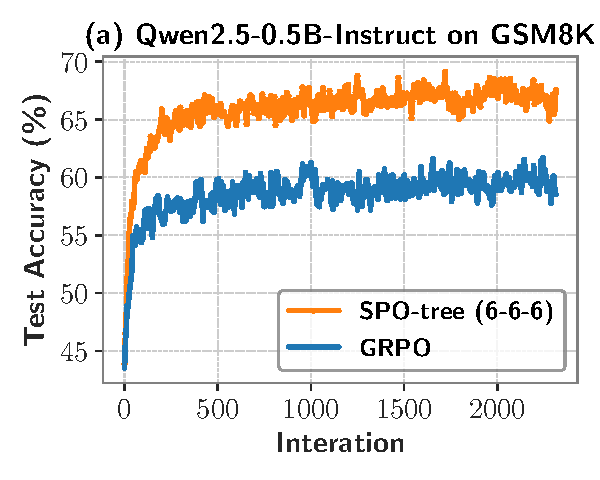
\includegraphics[width=\linewidth]{eval-figures/Qwen2.5-0.5B-Instruct.pdf}
  \label{fig:Qwen2.5-0.5B-Instruct}
\end{subfigure}
\hfill
\begin{subfigure}{0.48\textwidth}
  \centering
  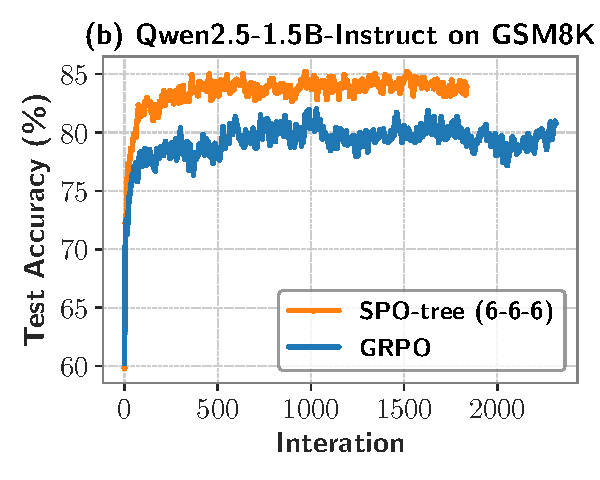
\includegraphics[width=\linewidth]{eval-figures/Qwen2.5-1.5B-Instruct.pdf}
  \label{fig:Qwen2.5-1.5B-Instruct}
\end{subfigure}

\begin{subfigure}{0.48\textwidth}
  \centering
  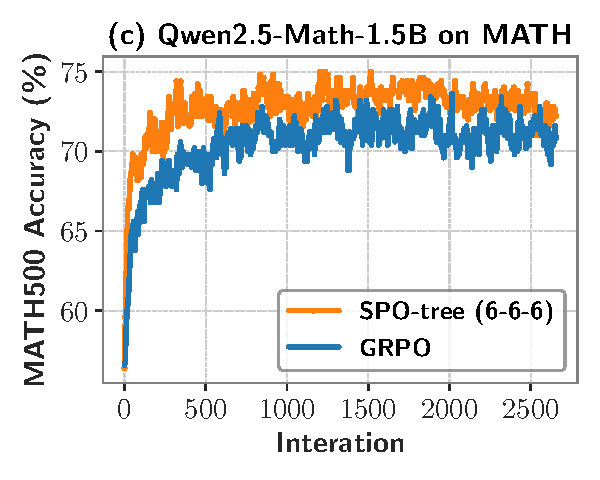
\includegraphics[width=\linewidth]{eval-figures/Qwen2.5-1.5B-Math.pdf}
  \label{fig:Qwen2.5-1.5B-Math}
\end{subfigure}
\hfill
\begin{subfigure}{0.48\textwidth}
  \centering
  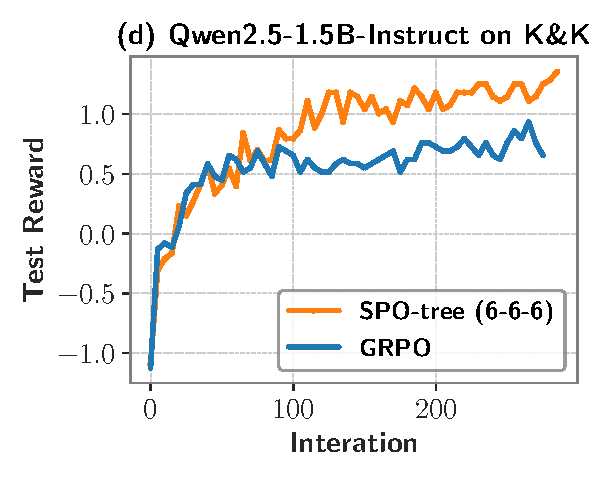
\includegraphics[width=\linewidth]{eval-figures/Qwen2.5-1.5B-Instruct-kk.pdf}
  \label{fig:kk}
\end{subfigure}

\caption{Experimental results across different models and datasets. 
(a) Qwen2.5-0.5B-Instruct on GSM8K. 
(b) Qwen2.5-1.5B-Instruct on GSM8K. 
(c) Qwen2.5-1.5B-Math on MATH. 
(d) Qwen2.5-1.5B-Instruct on Knights-and-Knaves (3ppl).}
\label{fig:more_experiments}
\end{figure*}